	%%%%%%%%%%%%%%%%%%%%%%%%%%EJERCICIO 13 %%%%%%%%%%%%%%%%%%%%%%%%%%%%%%%%%%%%%%%%%%%%%%%%%%%%%%
    \textbf{Ejemplo 13}\\
	
	Una cuota inicial del 30\% y el saldo será pagadero al final de 3 años, mientras tanto se pagarán intereses por período mes anticipado al 3\%. Con el objeto de cancelar la deuda a su vencimiento, se constituye un fondo que paga el 33\% nominal anual mes vencido mediante depósitos mensuales ordinarios crecientes en 2.000 COP. Determinar el costo del período 15.\\
	
	\textbf{Solución 13}\\
	%La tabla ira centrada
	\begin{center}
		\renewcommand{\arraystretch}{1.5}% Margenes de las celdas
		%Creación de la cuadricula de 3 columnas
		\begin{longtable}[H]{|p{0.5\linewidth}|p{0.5\linewidth}|}
			%Creamos una linea horizontal
			\hline
			%Definimos el color de la primera fila
			\rowcolor[HTML]{FFB183}
			%%%%% INICIO ASIGNACIÓN período FOCAL %%%%%%%
			%%%%%%%%%% INICIO TITULO
			%Lo que se hace aquí es mezclar las 3 columnas en una sola
			\multicolumn{2}{|c|}{\cellcolor[HTML]{FFB183}\textbf{1. Asignación período focal}}   \\ \hline
			%%%%%%%%%% FIN TITULO
			%%%%% INICIO DECLARACIÓN DE VARIABLES %%%%%%%
			\multicolumn{2}{|c|}{$pf = 36 \textit{ pmv}$}\\ \hline
			%%%%%%%%%% INICIO TITULO
			%Lo que se hace aquí es mezclar las 3 columnas en una sola
			\multicolumn{2}{|c|}{\cellcolor[HTML]{FFB183}\textbf{2. Declaración de variables}}   \\ \hline
			%%%%%%%%%% FIN TITULO
			%%%%%%%%%% INICIO DE MATEMÁTICAS
			%Cada & hace referencia al paso de la siguiente columna
			$  Interés = 4.200.000 \ COP (0,03) = 126.000 \ COP $  			 \\ \hline
			%%%%%%%%%% FIN DE MATEMÁTICAS
			%%%%% FIN DECLARACIÓN DE VARIABLES
			
			\rowcolor[HTML]{FFB183}
			\multicolumn{2}{|c|}{\cellcolor[HTML]{FFB183}\textbf{3. Diagrama de flujo de caja}} \\ \hline
			\multicolumn{2}{|c|}{ 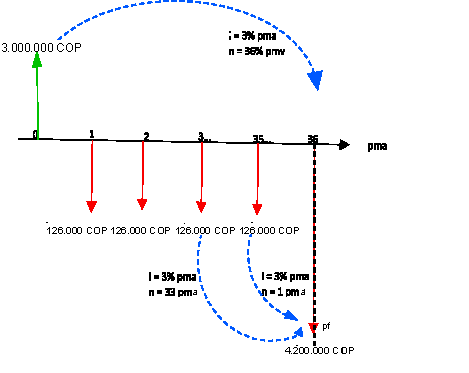
\includegraphics[trim=-78 -5 -78 -5]{7_Capitulo/img/ejemplos/13/13_1.pdf} }   \\
			\multicolumn{2}{|c|}{ 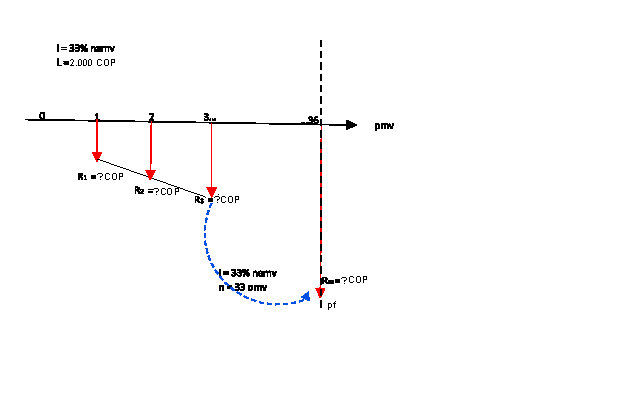
\includegraphics[trim=-78 -5 -78 -5]{7_Capitulo/img/ejemplos/13/13_2.pdf} }   \\ \hline
			%%%%% INICIO FLUJO DE CAJA
			\rowcolor[HTML]{FFB183}
			\multicolumn{2}{|c|}{\cellcolor[HTML]{FFB183}\textbf{4. Declaración de fórmulas}} \\ \hline
			%%%%%%%%%%%%% FIN INSERCIÓN DE IMAGEN
			%%%%%FIN FLUJO DE CAJA
			\multicolumn{2}{|c|}{ $VF = R n(1+i)^{n-1} $ \hspace{1mm} Formula del valor futuro gradiente geométrico si g=i}\\    
			\multicolumn{2}{|c|}{ $R_{n} = R_{1} + (n-1)L $ \hspace{1mm} Valor de un periodo aritmetico en un periodo n}   \\ \hline
			
			%%%%%% INICIO DESARROLLO MATEMÁTICO
			\rowcolor[HTML]{FFB183}
			%%%%%%%%%%INICIO TITULO
			\multicolumn{2}{|c|}{\cellcolor[HTML]{FFB183}\textbf{5. Desarrollo matemático}}       \\ \hline
			%%%%%%%%%% FIN TITULO
			%%%%%%%%%% INICIO MATEMÁTICAS
			\multicolumn{2}{|c|}{  $ 4.200.000 \ COP = R_{1} (36) (0,0275) + \frac{ 2.000 \ COP }{0,0275} ((36)(0,0275)-36) $}   \\ 
			\multicolumn{2}{|c|}{  $  R_{1} = 40.531,73 \ COP $}   \\ 
			\multicolumn{2}{|c|}{ $  R_{15} = 40.531,73 \ COP +  ( 15 - 1) (2.000 \ COP) = 68.531,73 \ COP $}   \\  \hline
			
			%%%%%%%%%% FIN MATEMÁTICAS
			%%%%%% FIN DESARROLLO MATEMÁTICO
			%%%%%% INICIO RESPUESTA
			\rowcolor[HTML]{FFB183}
			%%%%%%%%%%INICIO TITULO
			\multicolumn{2}{|c|}{\cellcolor[HTML]{FFB183}\textbf{6. Respuesta}}   \\ \hline
			%%%%%%%%%% FIN TITULO
			%%%%%%%%%% INICIO RESPUESTA MATEMÁTICA
			%\multicolumn{2}{|c|}{ 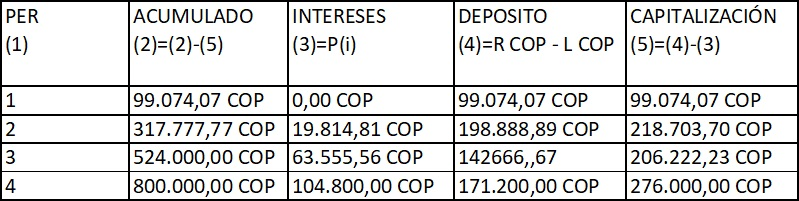
\includegraphics[trim=-78 -5 -78 -5]{7_Capitulo/img/ejemplos/12/12_2.jpg} }   \\ \hline
			\multicolumn{2}{|C{\textwidth}|}{
				$  R_{1} = 40.531,73 \ COP \hspace{2mm} y  \hspace{2mm} R_{15} = 68.531,73 \ COP $
				
				Esto significa que en el período 15 el deudor debe disponer de 194.531,73 COP de los cuales 126.000 COP los dedica al pago de intereses y el resto (68.531,73 COP) se deposita en el fondo.
				
			}  \\ \hline
			
			
			%%%%%%%%%% FIN MATEMÁTICAS
			%%%%%% FIN RESPUESTA
		\end{longtable}
		%Se crean dos lineas en blanco para que no quede el siguiente texto tan pegado
		%\newline \newline %USARLO SI CREES QUE ES NECESARIO
	\end{center}
%%%%%%%%%%%%%%%%%%%%%%%%%%FIN EJERCICIO 13